\apendice{Plan de Proyecto Software}

\section{Introducción}
En este anexo se va a exponer la planificación temporal y el estudio de viabilidad del proyecto.

Siguiendo la metodología Scrum, la planificación temporal está dividida en los \textit{sprints} seguidos para la realización del proyecto.
Cada apartado dentro de la planificación cuenta con información sobre la reunión de planificación del \textit{sprint}, de la que se obtienen conjunto de tareas a realizar, y la reunión de revisión, donde se muestra y valora el trabajo realizado.

\section{Planificación temporal}
Durante este proyecto se ha seguido una metodología Scrum con algunos cambios ya que no se hacían reuniones diarias ni los roles estaban tan marcados, pero la forma de trabajar era la misma con planificaciones y revisiones de \textit{sprints}.
Los \textit{sprints} que se han realizado son los siguientes:

\subsubsection{\textit{Sprint} 1: \textit{Sprint} inicial}
Fechas: 28 febrero 2023 -- 7 marzo 2023.
\begin{itemize}
\item\textbf{Planificación del \textit{sprint}}

En la reunión de planificación del sprint se fijaron las siguientes tareas:
\begin{enumerate}
	\item Configuración inicial del repositorio
	\item Prototipos de las vistas de la aplicación
	\item Creación diagrama entidad-relación
\end{enumerate}

\item\textbf{\textit{Burndown Report}}

\begin{figure}
	\centering
	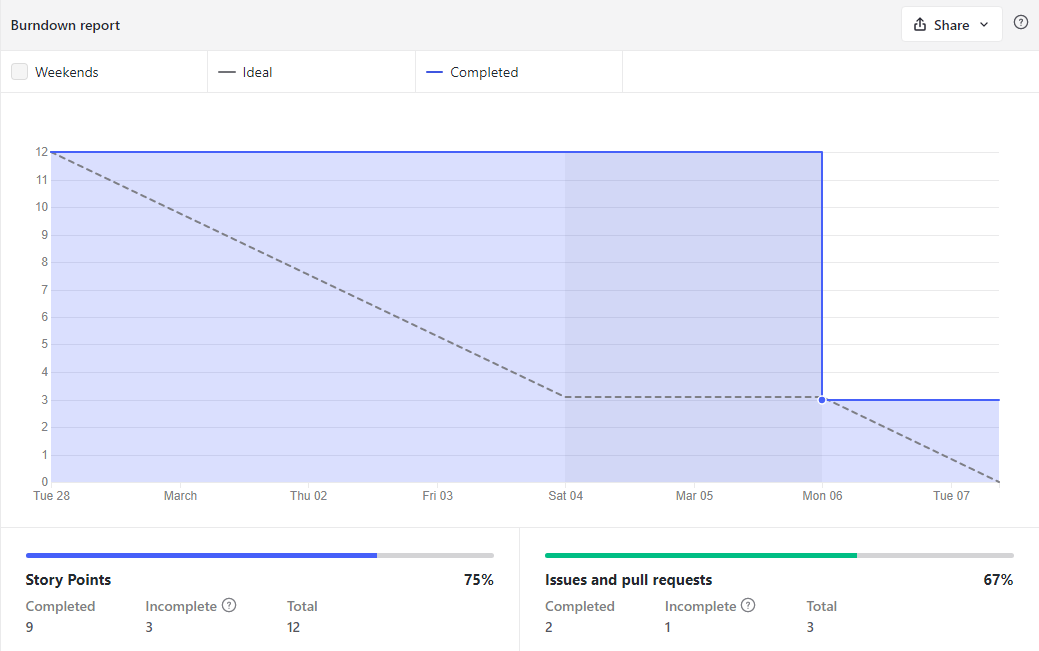
\includegraphics[width=\textwidth]{../img/Anexos/Sprints/Sprint1.png}
	\caption{\textit{Burndown Report Sprint 1}}\label{ReportSprint1}
\end{figure}

Como se puede apreciar en la figura~\ref{ReportSprint1}, no todas las tareas aparecen como completadas. Esto es debido a que el diagrama entidad-relación se dejó abierto ya que faltaba información para completarlo.

\item\textbf{Revisión del \textit{sprint}}

Durante la revisión se mostró el trabajo realizado y se vieron los cambios que se debían realizar en el diagrama entidad-relación que a su vez implicaban cambios en los prototipos de las vistas de la aplicación.
Se llegó a la conclusión de que podía ser buena idea dividir el diagrama E/R haciendo vistas del mismo para que fuere más fácil resolverlo.
\end{itemize}


\subsubsection{\textit{Sprint} 2: Casos de uso y diagrama E/R de cada uno}
Fechas: 7 marzo 2023 -- 14 marzo 2023.
\begin{itemize}
\item\textbf{Planificación del \textit{sprint}}

En la reunión de planificación del sprint se fijaron las siguientes tareas:
\begin{enumerate}
	\item Creación de casos de uso junto a su vista del diagrama E/R.
	\item Aprendizaje de Flask.
\end{enumerate}

\item\textbf{\textit{Burndown Report}}

\begin{figure}
	\centering
	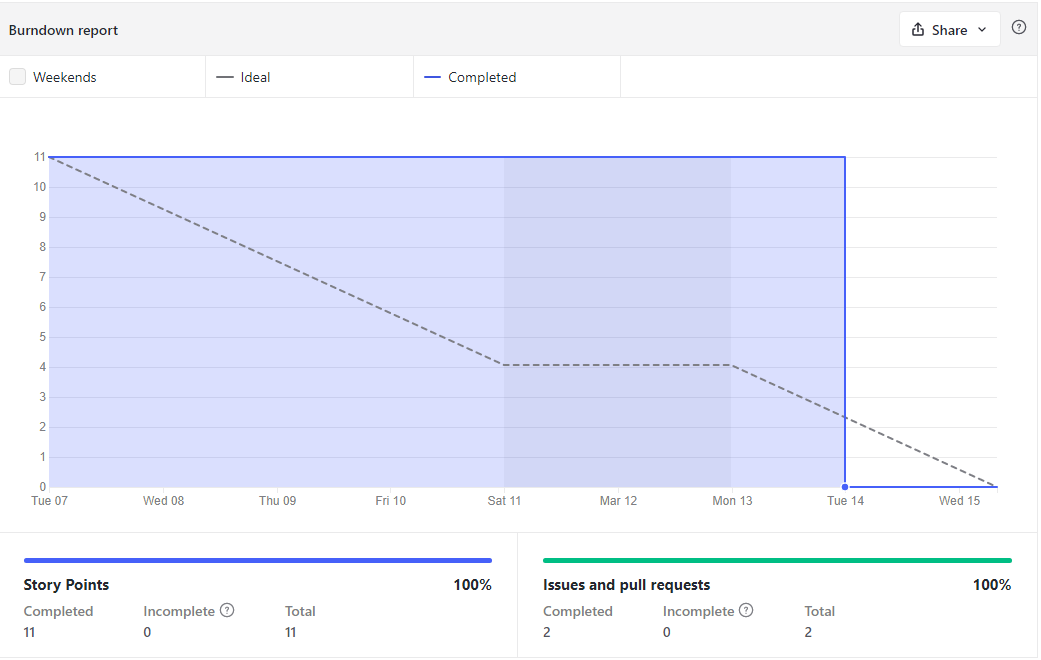
\includegraphics[width=\textwidth]{../img/Anexos/Sprints/Sprint2.png}
	\caption{\textit{Burndown Report Sprint 2}}\label{ReportSprint2}
\end{figure}

En este \textit{sprint} se completaron las tareas marcadas en el tiempo fijado durante la reunión de planificación, pero muchas cosas quedaron pendientes de cambios en futuros \textit{sprints}. En la figura~\ref{ReportSprint2} se puede ver el \textit{Burndown Report} del \textit{sprint}.

\item\textbf{Revisión del \textit{sprint}}

En la reunión de revisión se estudió de nuevo el diagrama E/R y se indicaron nuevos cambios menores en el mismo. También se propuso el comenzar a realizar el diagrama de casos de uso y continuar con el estudio de Flask.
\end{itemize}

\subsubsection{\textit{Sprint} 3: Documentación de casos de uso e investigación y aprendizaje de Flask y bibliotecas JavaScript}
Fechas: 14 marzo 2023 -- 21 marzo 2023.
\begin{itemize}
\item\textbf{Planificación del \textit{sprint}}

En la reunión de planificación del sprint se fijaron las siguientes tareas:
\begin{enumerate}
		\item Realizar el diagrama de casos de uso
		\item Cambios en las vistas adaptándolas a los casos de uso
		\item Documentar los casos de uso con sus tablas
		\item Investigar bibliotecas de JavaScript que pudiesen ayudar
		\item Aprender sobre Flask
\end{enumerate}

\item\textbf{\textit{Burndown Report}}

\begin{figure}
	\centering
	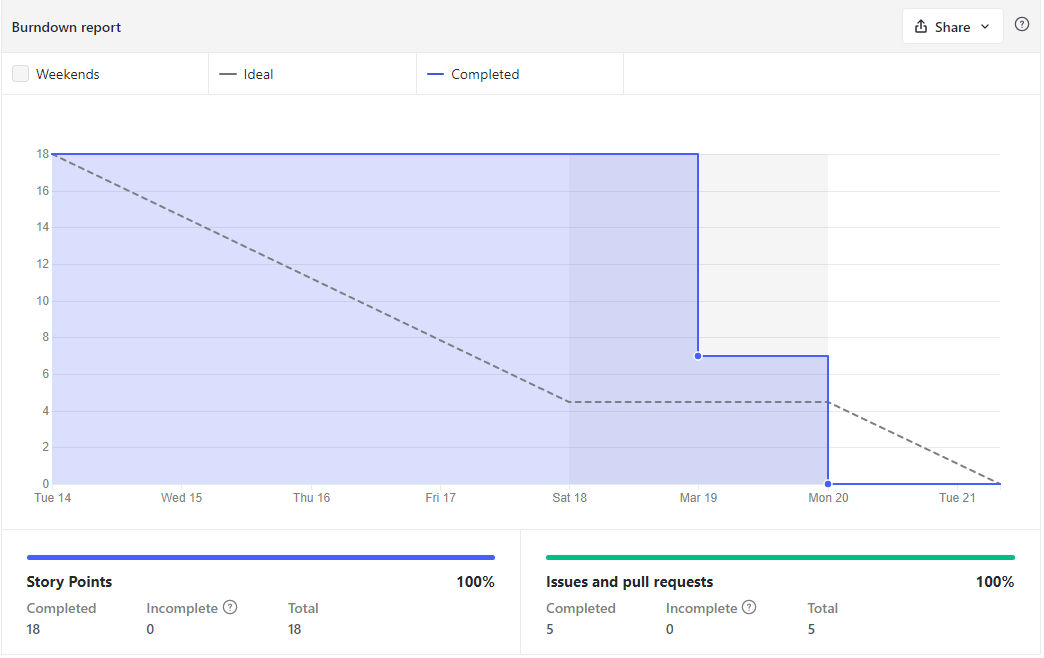
\includegraphics[width=\textwidth]{../img/Anexos/Sprints/Sprint3.png}
	\caption{\textit{Burndown Report Sprint 3}}\label{ReportSprint3}
\end{figure}

En este \textit{sprint} se completaron las tareas marcadas aunque el tiempo marcado para el aprendizaje de Flask fue menor debido a falta de tiempo durante esta semana. Estaba previsto dedicar en total 18 horas al \textit{sprint}, pero finalmente fueron 15. En la figura~\ref{ReportSprint3} se puede ver el \textit{Burndown Report} del \textit{sprint}.

\item\textbf{Revisión del \textit{sprint}}

Durante la revisión se vio que había casos de uso que no eran necesarios y que se podían añadir como excepciones de otros. Esto produjo que el diagrama de casos de uso se debía cambiar, lo que implica un cambio en la documentación de las tablas y en los prototipos de las vistas de la aplicación.
\end{itemize}

\subsubsection{\textit{Sprint} 4: Cambios en los casos de uso y vistas, documentación y Flask}
Fechas: 21 marzo 2023 -- 28 marzo 2023.
\begin{itemize}
\item\textbf{Planificación del \textit{sprint}}

En la reunión de planificación del sprint se fijaron las siguientes tareas:
\begin{enumerate}
		\item Cambios en el diagrama de casos de uso dividiendo en diagrama por niveles y crear vistas del diagrama E/R para los casos de uso.
		\item Cambios en algunos prototipos de las vistas de la aplicación.
		\item Cambios en la documentación de los casos de uso (tablas).
		\item Añadir documentación.
		\item Comenzar estructura básica de la aplicación en Flask.
\end{enumerate}

\item\textbf{\textit{Burndown Report}}

\begin{figure}
	\centering
	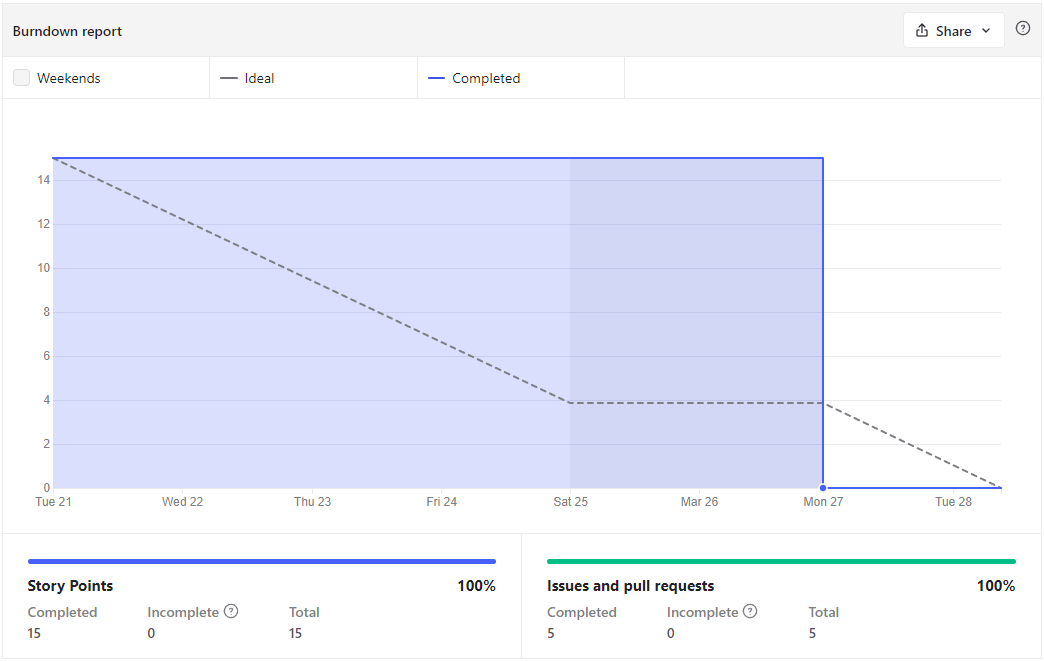
\includegraphics[width=\textwidth]{../img/Anexos/Sprints/Sprint4.png}
	\caption{\textit{Burndown Report Sprint 4}}\label{ReportSprint4}
\end{figure}

A lo largo del \textit{sprint} se realizaron la mayoría de tareas marcadas, pero en las tareas de añadir documentación y comenzar con Flask, no se hizo tanto como estaba esperado debido a la falta de tiempo. 
Se planeo que se iban a poder dedicar más horas de las que al final se dedicaron y no se avanzó todo lo planeado en estas tareas. 
Aún así, se decidió cerrarlas, ya que algo si se había avanzado, y crear de nuevo tareas similares en próximos \textit{sprints}.

La tarea de <<Cambios en el diagrama de casos de uso dividiendo en diagrama por niveles y crear vistas del diagrama E/R para los casos de uso>> tenía una previsión de 2 horas que se realizó en el plazo estimado, la tarea <<Cambios en algunos prototipos de las vistas de la aplicación>> tenía una estimación de 3 horas aunque finalmente fueron 4, la tarea <<Cambios en la documentación de los casos de uso (tablas)>> tenía marcada 4 horas de duración que finalmente fueron 5, la tarea de <<Añadir documentación>> tenía pensada una dedicación de 3 horas que al final se quedó en 1 hora y media aproximadamente y, por último, la tarea <<Comenzar estructura básica de la aplicación en Flask.>> tenía una previsión de 3 horas que quedó reducida a una media hora por falta de tiempo durante el \textit{sprint}. 
En la figura~\ref{ReportSprint4} se puede ver el \textit{Burndown Report} del \textit{sprint}.

\item\textbf{Revisión del \textit{sprint}}

En la reunión de revisión del \textit{sprint} se decidió hacer algunos cambios en los casos de uso, lo que implica un cambio en la documentación de las tablas y los prototipos de las vistas ya que el funcionamiento esperado de la aplicación cambia. También se decidió realizar algún cambio en el diagrama E/R añadiendo nuevos atributos y sacando un atributo a una nueva entidad.
\end{itemize}

\subsubsection{\textit{Sprint} 5: Documentación y comienzo de la aplicación}
Fechas: 28 marzo 2023 -- 11 abril 2023.
\begin{itemize}
\item\textbf{Planificación del \textit{sprint}}

En la reunión de planificación del sprint se fijaron las siguientes tareas:
\begin{enumerate}
		\item Cambios en el diagrama E/R y en algún caso de uso.
		\item Cambios en algunas tablas de los CU y en sus respectivas vistas.
		\item Evaluar plugins/frameworsk para tablas.
		\item Añadir documentación.
		\item Desarrollo de la aplicación.
\end{enumerate}

\item\textbf{\textit{Burndown Report}}

En este \textit{sprint} surgió un problema con herramienta ZenHub que utilizaba para llevar un seguimiento de los \textit{sprints} desde GitHub. Es una herramienta de pago que en teoría cuenta con versiones gratuitas para proyectos \textit{open source} y para profesores. Contacté con ellos para poder obtener una licencia gratuita de la herramienta, pero no fue posible conseguirla. Por lo tanto, a partir de este \textit{sprint} no pude utilizar la herramienta y no pude sacar la imagen del \textit{Burndown Report}.

Para la tarea de <<Cambios en el diagrama E/R y en algún caso de uso>> se estimaba un tiempo de realización de 1 hora que se cumplió.

Para la tarea <<Cambios en algunas tablas de los CU y en sus respectivas vistas>> se puso una estimación de 5 horas que finalmente fueron 7 horas.

Para la tarea <<Evaluar plugins/frameworsk para tablas>> se había marcado una planificación de 2 horas que se cumplió, excediendo un poco de la planificación, ya que aparte de buscar y valorar distintas librerías de JavaScript para la visualización de tablas estuve haciendo pruebas con la librería Grid.js que decidí utilizar para el proyecto.

La tarea de <<Añadir documentación>> tenía marcada una planificación de 3 horas que se cumplió dentro del plazo.

Por último, la tarea de <<Desarrollo de la aplicación>>, donde se buscaba empezar con la aplicación web, tenía una estimación de 8 horas que se convirtió en unas 10 horas de trabajo real debido a algunos problemas surgidos durante el desarrollo.

\item\textbf{Revisión del \textit{sprint}}

En la reunión de revisión se estuvo viendo el trabajo realizado durante el \textit{sprint}. En la parte de documentación se decidió que se debían hacer algunos pequeños cambios en las tablas de los casos de uso, la visualización de imágenes, cambios de orden en un diagrama y cambios en algún título.

En la parte de desarrollo de la aplicación web se decidió realizar algunos cambios en la visualización de tablas para que no ocupasen tanta pantalla así como en el menú de la web para hacerlo más pequeño introduciendo submenús. También se dijo que era mejor poner un selector de centro en la pantalla de la asignación de horas para que de esta forma ya saliesen los datos de la tabla filtrados por centro. 
\end{itemize}

\subsubsection{\textit{Sprint} 6: Base de datos y comenzar a dar funcionalidad a la web}
Fechas: 11 abril 2023 -- 24 abril 2023.
\begin{itemize}
\item\textbf{Planificación del \textit{sprint}}

En la reunión de planificación del sprint se fijaron las siguientes tareas:
\begin{enumerate}
		\item Creación de los modelos y la base de datos en base a los modelos.
		\item Crear la primera carga de la base de datos con CSV y script SQL.
		\item Creación de más vistas junto a su funcionalidad.
		\item Cambios en la documentación.
		\item Añadir más documentación.
\end{enumerate}

\item\textbf{\textit{Burndown Report}}

Este \textit{sprint} tenía una duración inicial de una semana, pero debido a falta de tiempo por exámenes y entregas de trabajos, decidí aplazar una semana más la reunión de revisión para poder trabajar en el proyecto. 
Además, se tuvo que cambiar la fecha habitual de las reuniones debido a que empecé prácticas en una empresa y ya no era compatible la hora/día que se tenía.

La primera tarea completada fue la de <<Creación de los modelos y la base de datos en base a los modelos>>. 
Se puso una estimación de 4 horas, que de trabajo real fue el doble, unas 8 horas. 
Este exceso de tiempo fue debido en gran medida a errores surgidos a la hora de crear la base de datos utilizando el \textit{ORM} SQLAlchemy. 
Los problemas eran principalmente por como hacía la carga de la base de datos que hacía que en algunos contextos estuviese disponible y en otros no, provocando errores al ejecutar la aplicación y generar las tablas de la base de datos.

La tarea <<Crear la primera carga de la base de datos con CSV y script SQL>> tenía una planificación de 2 horas y se completó en el tiempo. 
Sólo quedo pendiente el hecho de que desde la interfaz phpMyAdmin que estoy utilizando para manejar la base de datos, no fui capaz de cargar los archivos csv desde el script de SQL y tuve que cargarlos por separado desde la interfaz.

Para la tarea <<Creación de más vistas junto a su funcionalidad>> se tenía una estimación de 6 horas. 
En este caso fui bastante optimista y el trabajo real termino siendo de 9 horas.
Esto se debido en gran parte a la aparición de problemas que hicieron que tuviera que trabajar más horas de las planeadas en esta tarea.

La tarea <<Cambios en la documentación>> tenía planificadas 2 horas de trabajo. 
En horas reales termino siendo 2 horas y media aproximadamente.

Finalmente, la tarea de <<Añadir más documentación>> tenía una estimación de 1 hora y el trabajo realizado fue también de 1 hora. 
Se añadió sobre todo documentación sobre técnicas y herramientas, apartado de diseño y apartado de plan de proyecto.

\item\textbf{Revisión del \textit{sprint}}

En la reunión de revisión del \textit{sprint} 6 se estuvieron valorando los cambios realizados y las nuevas funcionalidades añadidas.
También se resolvieron algunas dudas sobre la documentación y algunas partes de la funcionalidad de la aplicación web.
Se discutieron algunos aspectos como el añadir algún nuevo campo en la base de datos para códigos internos o cómo tratar la eliminación de los centros, que hasta ahora se trataba como una eliminación en cascada, y se decidió cambiar al existir demasiado riesgo de pérdida de información por un borrado accidental o poco planificado.

\end{itemize}


\subsubsection{\textit{Sprint} 7: Creación de CRUDs y documentar}
Fechas: 24 abril 2023 -- 2 mayo 2023.
\begin{itemize}
\item\textbf{Planificación del \textit{sprint}}


En la reunión de planificación del sprint se fijaron las siguientes tareas:
\begin{enumerate}
		\item Comentarios sobre memoria y anexos.
		\item Crear el CRUD\footnote{CRUD son las siglas de \textit{Create} (crear), \textit{Read} (leer), \textit{Update} (actualizar) y \textit{Delete} (modificar).} de Docentes, Plazas, Contratos, Áreas y Departamentos.
		\item Solucionar bug con las abreviaturas al modificar una asignatura.
		\item Algunos cambios en campos de la base de datos.
		\item Buscar cómo cargar un CSV desde un script de SQL en phpMyAdmin.
		\item Añadir documentación.
\end{enumerate}

\item\textbf{\textit{Burndown Report}}

La tarea de <<Comentarios sobre memoria y anexos>> fue una tarea creada por Álvar Arnaiz González para dejar las correcciones hechas en la memoria y los anexos. 
Esta tarea fue reutilizada para indicar que se iban a subir esos cambios en la documentación. 
Tenía una planificación de 30 minutos y se realizó dentro del tiempo estimado.

La tarea <<Crear el CRUD de Docentes, Plazas, Contratos, Áreas y Departamentos>> era la que tenía más carga de trabajo en este \textit{sprint} con una estimación de 8 horas que se convirtió en 11 horas de trabajo real.
Este incremento de horas se debió principalmente a problemas para configurar correctamente la biblioteca Select2 utilizando Ajax y para mantener las opciones marcadas en el campo en las modificaciones.

La tarea <<Solucionar bug con las abreviaturas al modificar una asignatura>> era debida a errores en el campo \texttt{Select2} al hacer una modificación de una asignatura. 
Las abreviaturas de la asignatura aparecían bien, pero no se recuperaban de forma correcta en el servidor para saber cuales habían sido añadidas o eliminadas.
Esta tarea tenía una estimación de 1 hora y no se pretendía superar ese tiempo de trabajo, ya que en la reunión de planificación no se consideró que fuese un problema crucial debido a que en este momento no era necesario que una asignatura tuviera varias abreviaturas y podía ser cambiado por un campo de texto normal que no diese ese problema y permitiese a una asignatura tener una única abreviatura.
Al realizar la tarea anterior se tuvo un problema parecido que dio la pista para resolver este problema dejándolo totalmente subsanado.

La tarea <<Algunos cambios en campos de la base de datos>> tenía una estimación de 1 hora y se realizó dentro del plazo.
La tarea consistía en añadir nuevos campos en la base de datos, lo que suponía también hacer cambios en el código para introducir los nuevos atributos en los modelos y en los formularios.
También se cambió el borrado en cascada que tenían los centros para evitar que se eliminen centros que tengan titulaciones vinculadas.

Para la tarea <<Añadir documentación>> se estimaron 3 horas de trabajo que se cumplieron en cuanto a trabajo real.

Finalmente, para la tarea <<Buscar cómo cargar un CSV desde un script de SQL en phpMyAdmin>> se estimó 1 hora de trabajo que finalmente fue un trabajo real de 2 horas debido a que tuve que investigar por los problemas que me daba con la carga de los ficheros csv. El problema finalmente fue donde estaban colocados los csv.


\item\textbf{Revisión del \textit{sprint}}

En la reunión de revisión se mostró el trabajo realizado y se resolvieron algunas dudas acerca de la memoria y algunas partes del funcionamiento de la aplicación web.
\end{itemize}


\subsubsection{\textit{Sprint} 8: Gestión de cursos}
Fechas: 2 mayo 2023 -- 15 mayo 2023.
\begin{itemize}
\item\textbf{Planificación del \textit{sprint}}


En la reunión de planificación del sprint se fijaron las siguientes tareas:
\begin{enumerate}
		\item Subir la web a Heroku.
		\item Programar el apartado ge gestión de cursos.
		\item Hacer pequeños cambios en la web.
		\item Añadir documentación de trabajos relacionados.
\end{enumerate}

\item\textbf{\textit{Burndown Report}}

La primera tarea que se realizó fue <<Subir la web a Heroku>>.
La tarea tenía una carga de trabajo estimada en 2 horas.
Para esta tarea la estimación no fue nada correcta, ya que el trabajo real fue aproximadamente de 8 horas.
Esto fue debido principalmente a problemas a la hora de configurar el proyecto para ser reconocido por la plataforma Heroku y para configurar correctamente la base de datos. 
Surgieron un gran listado de problemas que fueron resueltos uno por uno hasta que la instalación fue satisfactoria.

Para la tarea <<Programar el apartado ge gestión de cursos>> se habían marcado 8 horas de trabajo que finalmente se convirtieron en mucho más, 20 horas de trabajo.
Esta gran discrepancia entre la planificación y el trabajo real fue debida en gran medida a la investigación y planteamiento de cómo mostrar el listado de asignaturas que se deben seleccionar a la hora de crear un curso.
Se intentó crear de la forma más cómoda para utilizar y con el menor impacto posible en el rendimiento.
También surgieron algunos problemas durante la programación que fueron subsanados pero que hicieron que el tiempo de trabajo se fuese desplazando aun más de la estimación realizada.

La siguiente tarea fue <<Hacer pequeños cambios en la web>>.
Esta tarea tenía una estimación de 3 horas que de trabajo real en realidad fueron unas 2 horas. 
Estos pequeños cambios eran principalmente sobre la visualización del contenido.

Finalmente, la tarea <<Añadir documentación de trabajos relacionados>> tenía una estimación de trabajo de 1 hora y el trabajo real tuvo también una duración aproximada de una hora.


\item\textbf{Revisión del \textit{sprint}}

Durante la reunión de revisión se vieron principalmente los cambios realizados en la web. Se estuvieron discutiendo diferentes formas de crear los cursos y se llegó a la conclusión de hacer pequeños cambios para que fuese más cómoda la creación de cursos.
También se estuvieron viendo las diferentes secciones de la memoria para dar ideas sobre la documentación que se podía ir introduciendo.
\end{itemize}


\subsubsection{\textit{Sprint} 9: Cambios, gestión de grupos y documentación}
Fechas: 15 mayo 2023 -- 23 mayo 2023.
\begin{itemize}
\item\textbf{Planificación del \textit{sprint}}


En la reunión de planificación del sprint se fijaron las siguientes tareas:
\begin{enumerate}
		\item Algunos cambios en la gestión de cursos.
		\item Creación de la gestión de grupos.
		\item Pequeños cambios/mejoras en el código.
		\item Avanzar en la memoria.
\end{enumerate}

\item\textbf{\textit{Burndown Report}}

Para la tarea <<Algunos cambios en la gestión de cursos>> se fijaron 4 horas. 
Esta tarea tenía como propósito realizar los cambios vistos en la reunión de revisión del \textit{sprint} anterior.
Estos cambios llevaron unas 3 horas de trabajo, pero debido a algunos errores al realizar los cambios se consumieron las 4 horas planificadas.

La segunda tarea realizada fue <<Creación de la gestión de grupos>>.
En esta tarea se quería crear todo lo relacionado con la gestión de grupos.
Desde su visualización en una tabla, a la creación y eliminación de los mismos para cada asignatura de un curso académico.
Para esta tarea se dio una estimación de 8 horas que en trabajo real fueron algo menos, pero cercano a las 8 horas.

La tercera tarea de <<Pequeños cambios/mejoras en el código>> tenía una estimación de tiempo de 1 hora y se cumplió en este tiempo.
En esta tarea se realizaron algunos cambios menores de diseño, cambios en vistas, algunos pequeños cambios de lógica, etc.

Finalmente, la tarea de <<Avanzar en la memoria>> tenía una estimación de 3 horas.
En esta tarea se pretendían realizar los cambios vistos en la documentación y añadir nueva información a la memoria.
La tarea llevó un trabajo real de aproximadamente las 3 horas. Se hicieron avances en la memoria y se añadió en los anexos el diccionario de datos, además de realizar los cambios vistos por toda la documentación.

\item\textbf{Revisión del \textit{sprint}}

En la reunión del \textit{sprint} 9 se estuvieron viendo los avances realizados. Se comentó que podría ser buena idea realizar algunos cambios en la creación de grupos y añadir una vista donde visualizar las titulaciones de un centro y las asignaturas de una titulación. Además, se descubrió un error en la eliminación de grupos y se estuvo hablando sobre como realizar el inicio de sesión de la aplicación a través de un \textit{token} devuelto por Moodle.
\end{itemize}

\subsubsection{\textit{Sprint} 10: Asignación de horas}
Fechas: 23 mayo 2023 -- 29 mayo 2023.
\begin{itemize}
\item\textbf{Planificación del \textit{sprint}}

En la reunión de planificación del sprint se fijaron las siguientes tareas:
\begin{enumerate}
		\item Crear la asignación de horas de plazas a grupos.
		\item Añadir forma avanzada de creación de grupos.
		\item Arreglar la eliminación de grupos.
		\item Cambios de campos obligatorios en <<Añadir Plaza>>.
		\item Arreglo \textit{bug} de números negativos.
		\item Mejoras de navegación en la web.
		\item Añadir documentación en los anexos.
\end{enumerate}

\item\textbf{\textit{Burndown Report}}

Para la tarea <<Crear la asignación de horas de plazas a grupos>> se fijaron 8 horas de trabajo.
La realidad fue un trabajo de aproximadamente 12 horas.
Este exceso de horas es debido a algunas complicaciones para realizar lo deseado que no se habían tenido en cuenta, pero que se fueron solucionando durante el desarrollo.

Para la tarea <<Añadir forma avanzada de creación de grupos>> se realizó una estimación de 4 horas.
Sin embargo, se dejó la tarea pausada hasta la próxima reunión debido a algunas incompatibilidades con el funcionamiento actual del sistema.
En la próxima reunión habrá que decidir si añadir esa funcionalidad cambiando las actuales o descartar la idea.

En la tarea <<Arreglar la eliminación de grupos>> se pretendía arreglar la reasignación de nombres de grupos al eliminar un grupo teórico.
En la creación de esta funcionalidad no se había probado bien y si se eliminaba un grupo teórico al que le pertenecían grupos prácticos, estos no se renombraban y daban lugar a futuros problemas.
Para la realización de la tarea se hizo una estimación de 2 horas y se realizó dentro de ese tiempo.

La tarea <<Cambios de campos obligatorios en "Añadir Plaza">> fue añadida por los tutores del proyecto al probar la aplicación y decidir realizar algunos cambios en los campos que debían ser obligatorios al crear una nueva plaza. 
Tenía una previsión de 15 minutos, pero estos pequeños cambios llevaron entre 20 y 30 minutos debido a que hubo que realizar cambios en la base de datos y, para ello, instalar y configurar una biblioteca para migraciones de la base de datos.

La tarea <<Arreglo \textit{bug} de números negativos>> también fue añadida por los tutores del proyecto al realizar sus pruebas en la web.
Algunos campos no se validaban bien y permitían ingresar números negativos en sitios donde esto no debía se posible.
Estos pequeños cambios llevaron aproximadamente 15 minutos.

La tarea <<Mejoras de navegación en la web>> fue otra de las añadidas por los tutores del proyecto.
Se pretendía mejorar la navegación por la web añadiendo botones de volver atrás sin realizar cambios en los formularios.
Además, se deseaba añadir una ventana desde donde ver las titulaciones de un centro y las asignaturas de una titulación.
Estos cambios tuvieron una estimación de poco más de una hora y, al final, el trabajo real también fue acorde.

Finalmente, para la tarea de <<Añadir documentación en los anexos>> se realizó una estimación de 3 horas.
Debido a falta de tiempo apenas se pudo avanzar y el trabajo real se quedó en aproximadamente media hora.


\item\textbf{Revisión del \textit{sprint}}

En la reunión del \textit{sprint} 10 se estuvieron viendo todos los cambios realizados.
En cuanto a la asignación de horas a plazas se dio el visto bueno, pero se propusieron algunos cambios en la visualización de los datos y se estudió la posibilidad de actualizar alguna información de la tabla mediante \textit{Ajax} al realizar una actualización sobre la misma.

Otro de los aspectos que fueron claves en la reunión fue la creación de grupos de forma avanzada indicando el nombre del grupo. Se llegó a la conclusión de que es una característica que podría ser interesante en un futuro aunque no primordial.
Además, de la forma que se había hecho el diseño era difícil adaptarlo y se decidió dejarlo como una característica interesante para próximas versiones de la aplicación.
\end{itemize}

\subsubsection{\textit{Sprint} 11: Pequeños cambios y arreglos}
Fechas: 29 mayo 2023 -- 5 junio 2023.
\begin{itemize}
\item\textbf{Planificación del \textit{sprint}}

En la reunión de planificación del sprint se fijaron las siguientes tareas:
\begin{enumerate}
		\item Arreglo de \textit{bug} de curso duplicado.
		\item Algunos cambios en la visualización de las horas de plazas en grupos.
		\item Crear el duplicado de la asignación de horas a grupos al duplicar el curso.
		\item Arreglo de \textit{bug} de dos plazas con el mismo docente.
		\item Creación de \textit{login}.
\end{enumerate}

\item\textbf{\textit{Burndown Report}}

Para la tarea <<Arreglo de \textit{bug} de curso duplicado>> se fijaron 30 minutos de trabajo.
La realidad fue un trabajo de aproximadamente el mismo tiempo.
Fue un trabajo sencillo ya que principalmente se basa en comprobar si ya existía un curso con ese año y no permitir crear otro con el mismo año.

La tarea <<Algunos cambios en la visualización de las horas de plazas en grupos>> tenía una estimación de 4 horas.
En esta tarea se pretendía realizar varios cambios en la tabla general de horas sobre como se mostraba la información de los docentes y también cambios dentro de la propia ventana de las plazas asignadas a una asignatura.
El trabajo real fue de 2 horas ya que llevó menos trabajo del pensado en un inicio.

En cuanto a la tarea de <<Crear el duplicado de la asignación de horas a grupos al duplicar el curso>> se puso una estimación de 2 horas.
En esta tarea se pretendía implementar en el duplicado de un curso académico la opción de duplicar también las asignaciones de horas de plazas a las asignaturas del curso.
La tarea llevó aproximadamente las 2 horas estimadas para su realización.

La tarea <<Arreglo de \textit{bug} de dos plazas con el mismo docente>> se estimó en una duración de media hora ya que tan solo era arreglar un pequeño fallo de funcionamiento en el que a un docente se le podía asignar más de una plaza sin que la plaza tuviese fecha de cese.
La idea del funcionamiento es que un docente pueda tener como máximo una plaza sin fecha de cese, es decir, una plaza activa al mismo tiempo.
La duración real fue de poco más de la media hora marcada inicialmente.

Por último, para la tarea <<Creación de \textit{login}>> se puso una estimación de 3 horas.
En esta tarea se implementó el \textit{login} de la aplicación, utilizando para ello el inicio de sesión contra el Moodle de la UBU, el cual devuelve un \textit{token} en caso de inicio de sesión correcto.
Para el inicio de sesión primero se debe verificar que el usuario exista en esta aplicación, si no, por mucho que exista en Moodle, no dejará entrar a la aplicación web.
Además de la creación del \textit{login} se tuvo que implementar la gestión de permisos en todas las acciones de la web para verificar si el usuario estaba identificado o no, y de esta forma dejarle manejar la web o redirigir a la ventana de inicio de sesión.

\item\textbf{Revisión del \textit{sprint}}

En la reunión del \textit{sprint} 11 se dio el visto bueno a los cambios realizados, pero se estuvieron viendo algunos cambios que podrían mejorar la visualización de las horas asignadas a plazas.

También se explicó cómo debían funcionar los permisos en la aplicación web diferenciando de usuarios con permisos de modificación o permisos de lectura. Además de la posibilidad de tener usuarios sin ningún tipo de permiso, caso que se dará cuando se de un docente de baja.

También se vieron diferentes mejoras que se podrían añadir si daba tiempo como un botón para exportar e importar la información de la base de datos, la creación de gráficos con los datos de las horas de asignaturas, etc.
\end{itemize}


\subsubsection{\textit{Sprint} 12: Últimos cambios aplicación}
Fechas: 5 junio 2023 -- 12 junio 2023.
\begin{itemize}
\item\textbf{Planificación del \textit{sprint}}

En la reunión de planificación del sprint se fijaron las siguientes tareas:
\begin{enumerate}
		\item Cambios en el login y creación de campos de lectura y escritura en docente.
		\item Cambios visuales en el apartado de horas.
		\item Creación de opción para importar y exportar la base de datos.
		\item Arreglo de \textit{bug} con los permisos de usuario.
		\item Pequeños cambios de funcionamiento general.
		\item Avanzar documentación.
\end{enumerate}

\item\textbf{\textit{Burndown Report}}

La tarea <<Cambios en el login y creación de campos de lectura y escritura en docente>> tenía una estimación de 3 horas.
En esta tarea lo que se quería hacer era la forma de hacer el \textit{login} y, además, añadir dos campos en la tabla docente para identificar si se tienen permisos de lectura, modificación o ambos, y así mostrar diferentes elementos o vistas según los permisos.
Este trabajo llevó finalmente 5 horas, algo más de lo previsto debido a algunos problemas con la forma de implementar los permisos que se vio que no era le mejor forma y se decidió cambiar de nuevo por una forma más eficiente.
Además, inicialmente se guardaban el \textit{token} y el id del docente en el lado del cliente, cosa que carece en gran medida de seguridad, ya que "robar" una \textit{cookie} es algo relativamente sencillo y esto podría provocar el acceso a la aplicación por usuarios no deseados.
Para solucionar esto, se hizo un cambio para almacenar los datos de la sesión en la base de datos. 
Además, los datos se guardan cifrados, lo que añade muchas más seguridad de esta información sensible.

Para la tarea de <<Cambios visuales en el apartado de horas>> se dió una estimación de 1 hora y el trabajo se realizó en ese tiempo.

En cuanto a la tarea <<Creación de opción para importar y exportar la base de datos>> fue una de las más complejas.
La estimación inicial fue de 3 horas ya que se pensó que iba a ser una tarea relativamente sencilla.
La tarea pretendía añadir una nueva funcionalidad a la web en la que se permite exportar el contenido de la base de datos e importar el contenido descargado previamente.
Esta funcionalidad es interesante pensando en la importación sencilla de los datos cuando se cree una nueva implantación de la web. 

En un principió se pensó que sería una tarea sencilla, pero a la hora de la verdad fue una tarea complicada ya que la conexión y lectura de la base de datos no era algo tan sencillo.
Había que controlar los diferentes tipos de datos y solventar algunos errores con la tabla de sesiones que contaba con información en binario y que se pensó que lo mejor era no exportar esa información ya que no es relevante.

De cara a la importación también llevó mucho tiempo debido a estudiar los diferentes ataques que se podían producir con esta funcionalidad, tanto en la subida del archivo a la web, como en las sentencias incluidas en el SQL.
Finalmente se decidió permitir únicamente las sentencias \textit{insert}, ya que la idea de la funcionalidad es únicamente añadir datos a la base de datos, y así evitar borrados o modificaciones no deseadas.

El trabajo final fue de unas 8 horas, bastante más de lo estimado.

Para la tarea <<Arreglo de \textit{bug} con los permisos de usuario>> se dio una estimación de 20 minutos ya que lo único que se quería hacer era limitar las capacidades de un usuario sin permisos dentro de la aplicación, prohibiéndoles el acceso incluso a la ventana principal.
Actualmente, un usuario sin permisos no puede pasar del inicio de sesión, donde se muestra un mensaje indicando la falta de permisos.

La tarea <<Pequeños cambios de funcionamiento general>> tenía una estimación de 1 hora.
Esta tarea estaba diseñada para realizar algunos cambios visuales o de funcionalidad en la web. Así como carga interna de bibliotecas o datos.
La duración real de la tarea también fue de 1 hora aproximadamente.

Por último, la tarea de <<Avanzar documentación>> tenía una estimación de 4 horas de trabajo que quedó en unas 3 horas de trabajo real donde se añadió documentación en los anexos.

\item\textbf{Revisión del \textit{sprint}}

En la reunión del \textit{sprint} 12 se estuvieron viendo los cambios realizados y se decidió realizar algunos cambios a la hora de importar los datos a la base de datos añadiendo una confirmación antes de importar y la visualización de los datos a importar.
También se encontró un error en el funcionamiento de las sesiones que debía ser subsanado y por último, se estuvieron viendo los cambios y posibles adiciones que se podían realizar en la documentación.
\end{itemize}


\subsubsection{\textit{Sprint} 13: Avances en la documentación y arreglos}
Fechas: 12 junio 2023 -- 19 junio 2023.
\begin{itemize}
\item\textbf{Planificación del \textit{sprint}}

En la reunión de planificación del sprint se fijaron las siguientes tareas:
\begin{enumerate}
		\item Campo de reducciones por defecto a 0.
		\item Solucionar bug con las sesiones en la base de datos.
		\item Crear carga masiva de datos.
		\item Cambios en la función de importar datos.
		\item Añadir documentación y solucionar errores vistos.
\end{enumerate}

\item\textbf{\textit{Burndown Report}}

Para la tarea <<Campo de reducciones por defecto a 0>> se dio una estimación de 10 minutos y se hizo en ese mismo tiempo. 
Esta tarea consistía un pequeño cambio en poner un valor mínimo de 0 ya marcado en el campo reducciones de el formulario de docentes para hacer más cómoda la introducción de datos.

La tarea <<Solucionar bug con las sesiones en la base de datos>> tenía una previsión de 3 horas de trabajo que se convirtieron en 8 horas reales.
Con esta tarea se buscaba arreglar un bug que hacía que las sesiones no se almacenasen en la base de datos.
Al poco de mirarlo se vio que era un problema por el orden de carga de la biblioteca, pero al hacer pruebas se detectó un error entre las sesiones y la sesión de SQLAlchemy que hacía que en las eliminaciones no se esperase al commit y las hiciese de forma directa.
Tras darle muchas vueltas y buscar mucha información sin ningún resultado y revisar que todo estaba correcto, se decidió descartar la idea de utilizar SQLAlchemy para guardar las sesiones porque todo parecía indicar ser un bug de la biblioteca.
Para poder seguir almacenando las sesiones en el servidor, se optó por guardarlas en el sistema de ficheros, cosa que en un principio dio problemas en Heroku, pero que se consiguió solucionar.

La tarea <<Crear carga masiva de datos>> fue propuesta por el tutor de proyecto Álvar Arnaiz Gonzalez para tener datos reales de los centros, titulaciones, asignaturas, etc. 
En un principio se pensó que con 2 horas de trabajo sería suficiente, pero la realidad fueron unas 6 horas debido a que el formato en el que podíamos obtener los datos no era el mismo que necesitábamos y esto implicaba tener que hacer varias modificaciones.

Para la tarea de <<Cambios en la función de importar datos>> se dio una estimación de 3 horas que se convirtieron en unas 7 horas de trabajo. Esto es debido a que se tuvo que crear una función de JavaScript que fuese capaz de leer un archivo SQL y extraer de él la información que se iba a introducir en la base de datos mostrándolo en forma de tabla en el HTML. También se creó un mensaje de confirmación antes de importar para evitar fallos y, por último, se modifico la función de Python encargada de la importación para mejorar la validación del fichero subido.

Finalmente, la tarea de <<Añadir documentación y solucionar errores vistos>> estaba creada para, como su nombre indica, avanzar con la documentación del trabajo y para corregir las cosas vistas en la reunión del \textit{sprint}. 
Tenía una estimación de 8 horas que se quedó en unas 5 o 6 de trabajo real. No se pudo avanzar más debido a la falta de tiempo ya que otras tareas habían consumido más de lo esperado. 
La tarea de dejó abierta para continuar con ella en el siguiente \textit{sprint}. 

\item\textbf{Revisión del \textit{sprint}}

En la reunión del \textit{sprint} 13 estuvimos viendo algunos pequeños errores vistos por los tutores.
También se vieron los cambios realizados y se comentó alguna cosa que podía añadir a la documentación.
\end{itemize}


\subsubsection{\textit{Sprint} 14: Arreglo de errores y documentación de anexos}
Fechas: 19 junio 2023 -- 26 junio 2023.
\begin{itemize}
\item\textbf{Planificación del \textit{sprint}}

En la reunión de planificación del sprint se fijaron las siguientes tareas:
\begin{enumerate}
		\item \textit{Bug}: El campo plazas lleva a horas.
		\item No permitir eliminar al docente que está en la sesión.
		\item No permitir eliminar titulaciones con asignaturas.
		\item Recarga de página tras cambio de grupos.
		\item Cambiar el id por el nombre en las \textit{breadcrumbs}.
		\item Mejorar interfaz de \textit{login}.
		\item \textit{Bug}: En la importación de datos permite cualquier fichero.
		\item Añadir documentación en los anexos.

\end{enumerate}

\item\textbf{\textit{Burndown Report}}

Para la tarea <<\textit{Bug}: El campo plazas lleva a horas>> se dio una estimación de aproximadamente 5 minutos y se realizó dentro del plazo estimado.
En esta tarea simplemente había que cambiar el enlace de la opción <<plazas>> de la página inicial que estaba llevando a la vista de horas y no a la de plazas.

La siguiente tarea, <<No permitir eliminar al docente que está en la sesión>> tenía como finalidad no permitir que el docente con la cuenta activa pudiese eliminar o cambiar los permisos de su propia cuenta.
Para realizar esta tarea se dio una estimación de media hora y se realizó en unos 20 minutos, algo menos de lo previsto.

La tarea de <<No permitir eliminar titulaciones con asignaturas>> estaba creada para quitar la posibilidad del borrado en cascada de asignaturas dependientes de una titulación al eliminar esta.
Para esta tarea se hizo una estimación de 30 minutos que se quedó en la mitad de trabajo real, unos 15 minutos.

Para la tarea <<Recarga de página tras cambio de grupos>> se puso una estimación de 1 hora, pero finalmente el trabajo real fue de unas 3 horas.
Se quería quitar la recarga al modificar los campos de una asignatura de un curso desde la vista principal de <<grupos>>.
Se preveía que iba a ser un trabajo menor, pero al tener que cambiar la forma de funcionar a hacer una petición mediante Ajax para evitar la recarga hubo que modificar la función del controlador prácticamente al completo y hubo que crear la función de JavaScript encargada de gestionar esta tarea.

Otra tarea que se realizó fue la de <<Cambiar el id por el nombre en las \textit{breadcrumbs}>>.
Se dio una estimación de media hora y se realizó dentro del plazo.
Era una tarea sencilla ya que sólo se debía cambiar el identificador por el nombre, pero al ser un cambio en tantas acciones de distintos controladores se tardó un poco en completar la tarea.

La tarea de <<Mejorar interfaz de \textit{login}>> pretendía mejorar un poco el diseño de la ventana del \textit{login} haciéndola menos minimalista al añadirle algún contenido como el logo o un pie de página.
Esta tarea tenía una estimación de media hora de trabajo, pero el trabajo real se fue hasta aproximadamente las 3 horas.
Esto es debido a que surgió un problema con el pie de página que no se mostraba al final de la página y hubo que estudiar como hacer que se mostrase abajo del todo aunque no hubiese contenido suficiente en la página para rellenar hasta ahí. 
Además, al probar en un dispositivo móvil se detecto que no se mostraba del todo bien así que se cambió el formato completo del \textit{login} para que se mostrase bien en dispositivos con pantallas más pequeñas.

Para la tarea <<\textit{Bug}: En la importación de datos permite cualquier fichero>> se fue muy optimista ya que se estimó en 1 hora y finalmente fueron unas 4 horas de trabajo.
En esta tarea se quería controlar mejor los archivos que se subían para hacer una importación en la base de datos ya que se detectó que era posible seleccionar cualquier fichero, aunque en el servidor si se comprobaba si era SQL y se permitía o no.
La idea era que mediante JavaScript se hiciese una primera validación para directamente no dejar enviar el archivo y no mostrar la visualización.

Otro de los errores detectados era que si se cambiaba el formato a otro archivo, por ejemplo convertir un PDF en un archivo SQL, se permitía subir pero saltaba una excepción al intentar ejecutar la importación.
Tras investigar se consiguió hacer una primera validación desde JavaScript para detectar estos archivos SQL mal formados y no permitir subirlos.
Además, en Python también se controló el posible error que podía saltar.

Finalmente, para la tarea <<Añadir documentación en los anexos>> se propuso trabajar 6 horas y al final se hicieron en torno a esas 6 horas planteadas inicialmente.

\item\textbf{Revisión del \textit{sprint}}

En la reunión del \textit{sprint} 14 se estuvieron viendo algunas mejoras para la documentación y los cambios realizados durante el \textit{sprint}.
Además, se discutieron algunas pequeñas modificaciones para la web que podrían hacer más sencilla la navegación para todos los usuarios.

Finalmente, se estuvieron resolviendo algunas dudas sobre algunas partes de la documentación de cara a la entrega final del proyecto.
\end{itemize}

\subsubsection{\textit{Sprint} 15: Finalizar documentación y últimos retoques}
Fechas: 26 junio 2023 -- 3 julio 2023.
\begin{itemize}
\item\textbf{Planificación del \textit{sprint}}

En la reunión de planificación del sprint se fijaron las siguientes tareas:
\begin{enumerate}
		\item Realizar casos de prueba.
		\item Incluir observaciones en <<Añadir plaza>>.
		\item Cambios en <<Asignación docente>>.
		\item Solucionar \textit{bug} en la tabla de horas.
		\item Realizar algunas modificaciones en la documentación.
		\item Hacer el manual de usuario.
		\item Documentar las conclusiones y líneas futuras.
		\item Últimos retoques de diseño.
\end{enumerate}

\item\textbf{\textit{Burndown Report}}

La tarea de <<Realizar casos de prueba>> es la primera que se completó.
Se había hecho una estimación de 4 horas que se convirtieron en unas 5 horas reales.
Durante esta tarea se probó la aplicación y se documentaron los casos de prueba realizados.

La siguiente tarea que se completó fue la de <<Incluir observaciones en ``Añadir plaza''>>.
Esta tarea fue creada para añadir un campo de observaciones donde poder escribir texto libre al crear o modificar plazas.

Se estimó una duración de media hora que se cumplió en el mismo tiempo estimado.

Para la tarea de <<Cambios en ``Asignación docente''>> se dio una estimación de 5 minutos, ya que se trataba simplemente de cambiar algún texto para hacer más sencilla la navegación.
La tarea se cumplió dentro del tiempo planeado.

Otra tarea que se realizó durante este último \textit{sprint} fue la de <<Solucionar \textit{bug} en la tabla de horas>>.

Al hacer pruebas en la aplicación se detectó que con algunos navegadores la modificación de las horas de las plazas asignadas a grupos desde la tabla no funcionaba del todo bien, ya que la escritura parecía realizarse de derecha a izquierda.

Tras investigar el problema, se vio que este se producía al hacer uso de una expresión regular para permitir sólo números. 
Algunos navegadores reiniciaban la posición del cursor al pasar la expresión regular, por lo que la solución fue guardar la posición del puntero antes de pasar la expresión regular y devolverlo a el lugar que tenía después de esto.

Esta tarea tenía una estimación de tiempo de 1 hora, pero finalmente fue completada en casi 2 horas.

Para la tarea <<Realizar algunas modificaciones en la documentación>> se planteó una estimación de 1 hora y, en trabajo real, fue aproximadamente el mismo tiempo.

En esta tarea se buscaba arreglar algunas erratas detectadas y añadir más información a la memoria.

Otra tarea que se realizó fue la de <<Hacer el manual de usuario>>, con una estimación de 5 horas, que finalmente se convirtió en unas 7 horas de trabajo real.

La tarea <<Documentar las conclusiones y líneas futuras>> tenía una estimación de 2 horas y se realizó en aproximadamente el ese tiempo.

Por último, la tarea de <<Últimos retoques de diseño>> se fijó en 2 horas de trabajo, pero en realidad tomó aproximadamente 3 horas. Esto se debió a que se realizaron cambios sobre la marcha sin tener una idea clara de cuántos cambios se requerirían.

\item\textbf{Revisión del \textit{sprint}}

Durante la reunión del \textit{sprint} 15, se revisaron todas las adiciones a la memoria y se discutieron algunos de los pequeños cambios realizados en el sitio web.

Durante esta última reunión, también se plantearon algunas mejoras adicionales para la documentación, con el objetivo de tener todo listo para su impresión y entrega.
\end{itemize}

\section{Estudio de viabilidad}
El estudio de viabilidad es una etapa esencial en el desarrollo de cualquier proyecto, ya que permite evaluar la viabilidad económica, técnica y operativa de la propuesta. 

En este apartado, se abordará el estudio de viabilidad del proyecto realizado.
Se analizarán los aspectos económicos y legales del proyecto con el objetivo de determinar su viabilidad y establecer las bases para su exitosa implementación.

\subsection{Viabilidad económica}
Para determinar la viabilidad económica del proyecto es necesario analizar los costes que tiene y los posibles beneficios que puede otorgar.

\subsubsection{Coste de personal}
Para tener en cuenta los costes del proyecto, lo primero en lo que nos debemos fijar es el coste del personal involucrado en el proyecto realizado.

En este caso, ha habido un único desarrollador \textit{junior} trabajando poco más de 4 meses dedicando aproximadamente 350 horas de trabajo en este periodo.

Se toma como salario medio de un programador \textit{junior} los 19000~€ brutos anuales\footnote{\url{https://www.glassdoor.es/Sueldos/programador-junior-sueldo-SRCH_KO0,18.htm}}.
Suponiendo un trabajo de 1826 horas anuales\footnote{\url{https://asesorias.com/empresas/normativas/laboral/jornada/horas-trabajo-anuales/}}, se obtiene un precio de 10,40~€ por cada hora de trabajo.
Teniendo en cuenta las 350 horas trabajadas * 10,40~$\frac{\text{€}}{hora}$ = 3640~€ totales, lo que es lo mismo que 910~€ mensuales brutos.

Una vez calculado el salario es importante tener en cuenta que la empresa debe pagar impuestos adicionales a esta base.
En primer lugar debe pagar un 23.60\% de la base como contingencias comunes, 5,50\% de desempleo, un 0,6\% como formación, un 0,2\% de cotización al Fondo de Garantía Salarial (FOGASA) y un 1,5\% por accidentes de trabajo y enfermedades profesionales\footnote{\url{https://getquipu.com/blog/cuanto-cuesta-contratar-un-trabajador/}}.

El total de lo que debe pagar la empresa por el salario mensual del trabajador se puede ver en la ecuación~\ref{eq:sueldo}.

\begin{equation}\label{eq:sueldo}
\frac{910~\frac{\text{€}}{mes}}{1 - (0.236 + 0.055 + 0.006 + 0.002 + 0.0150)} = 1326.53~ \frac{\text{€}}{mes}
\end{equation}

Finalmente, el salario durante los 4 meses de trabajo asciende al total de 1326,53~ $\frac{\text{€}}{mes}$ * 4 meses = 5306,12~€.


\subsubsection{Coste de \textit{hardware}}
Para el desarrollo del proyecto es necesario contar con cierto \textit{hardware}.
En este caso, se ha utilizado un ordenador con un procesador Intel Core i5-8600, 16 GB de memoria RAM, tarjeta gráfica NVIDIA GeForce GTX 1060 y 1,5TB de almacenamiento.
Es un ordenador tiene un valor de aproximado de 900€. En cuanto a periféricos y pantalla se estima un precio de 190~€.

Este conjunto de \textit{hardware} se amortizará en 4 años. El coste anual de amortización se puede ver en la ecuación~\ref{eq:hardware}.

\begin{equation}\label{eq:hardware}
\frac{1090~\text{€}}{4~\text{años}} = 272.5~\frac{\text{€}}{año}
\end{equation}

Teniendo en cuenta que la duración del proyecto ha sido de 4 meses, el coste durante estos meses del \textit{hardware} es de 90,83~€.

Por último, sobre el servidor donde desplegar la aplicación, pondremos un precio estimado de unos 80~€ mensuales para un servidor dedicado\footnote{\url{https://www.ovhcloud.com/es-es/bare-metal/prices/}}. Por lo tanto, el coste durante estos 4 meses es de 320~€.

\subsubsection{Coste de \textit{software}}
En este apartado vamos a exponer el coste del \textit{software} utilizado para el desarrollo del proyecto.

Para la realización de este proyecto se han utilizado bibliotecas gratuitas. 
El único coste adicional que puede tener es el del uso del IDE PyCharm, el cual tiene un coste mensual de 24,90~€ en su versión profesional, por lo que el coste durante los 4 meses de utilización es de 99,60~€.

\subsubsection{Recuento}
El recuento de estos costes durante los 4 meses de desarrollo del proyecto se puede ver en la tabla~\ref{table-A:economía}

\begin{table}
  \centering 
  \begin{tabular}{l r}
    \toprule
    \textbf{Concepto} & \textbf{Coste (€)} \\
    \midrule
    Personal & 5306,12 \\
	\textit{Hardware} & 410,83 \\
	\textit{Software} & 99,60\\
	\midrule
	\textbf{Total} & 5816,55 \\
	\bottomrule
  \end{tabular}
\caption{Total de costes durante el desarrollo del proyecto.}\label{table-A:economía}
\end{table}


\subsubsection{Beneficios}
Este proyecto ha sido desarrollado para ser implementado en un departamento de la Universidad de Burgos sin obtener de ello ningún tipo de beneficio, ya que se trata de una aplicación interna de la propia universidad realizada con carácter educativo.

\subsection{Viabilidad legal}
La viabilidad legal de un proyecto permite evaluar y garantizar el cumplimiento de las leyes y regulaciones vigentes, tanto en el desarrollo como en el uso de la aplicación.

\subsubsection{Licencias del software utilizado}

En la tabla~\ref{table-A:licencias} se puede ver el listado de bibliotecas y herramientas utilizadas junto a su licencia.

\begin{table}
\centering 
\begin{tabular}{|l|p{.15\textwidth}|p{.38\textwidth}|}
\hline
\textbf{Biblioteca/herramientas} & \textbf{Versión} & \textbf{Licencia} \\
\hline
\texttt{alembic} & 1.11.1 & MIT License \\
\texttt{asgiref} & 3.6.0 & BSD-2 License \\
\texttt{cachelib} & 0.10.2 & MIT License \\
\texttt{click} & 8.1.3 & BSD-3 License \\
\texttt{colorama} & 0.4.6 & BSD-3 License \\
\texttt{Django} & 4.2.1 & BSD-3 License \\
\texttt{djangoApiDec} & 1.7 & MIT License \\
\texttt{dnspython} & 2.3.0 & ISC License \\
\texttt{email-validator} & 2.0.0.post2 & MIT License \\
\texttt{Flask} & 2.2.3 & BSD-3 License \\
\texttt{Flask-Menu} & 0.7.2 & BSD License \\
\texttt{Flask-Migrate} & 4.0.4 & BSD License \\
\texttt{Flask-Session} & 0.5.0 & BSD License \\
\texttt{Flask-SQLAlchemy} & 3.0.3 & BSD-3 License \\
\texttt{Flask-WTF} & 1.1.1 & BSD-3 License \\
\texttt{greenlet} & 2.0.2 & MIT License \\
\texttt{gunicorn} & 20.1.0 & MIT License \\
\texttt{idna} & 3.4 & BSD License \\
\texttt{importlib-metadata} & 6.1.0 & Apache License 2.0 \\
\texttt{itsdangerous} & 2.1.2 & BSD License \\
\texttt{jieba} & 0.38 & MIT License \\
\texttt{Jinja2} & 3.1.2 & BSD-3 License \\
\texttt{Mako} & 1.2.4 & MIT License \\
\texttt{MarkupSafe} & 2.1.2 & BSD License \\
\texttt{mysqlclient} & 2.1.1 & GNU Library General Public License v2 \\
\texttt{ngram} & 4.0.3 & Apache License 2.0 \\
\texttt{pymongo} & 3.4.0 & Apache License 2.0 \\
\texttt{PyMySQL} & 1.0.3 & MIT License \\
\texttt{PyPrind} & 2.9.9 & MIT License \\
\texttt{requests} & 2.12.3 & Apache License 2.0 \\
\texttt{simplejson} & 3.10.0 & MIT License \\
\texttt{six} & 1.16.0 & MIT License \\
\texttt{SQLAlchemy} & 2.0.9 & MIT License \\
\texttt{sqlparse} & 0.4.4 & BSD License \\
\texttt{typing\_extensions} & 4.5.0 & MIT License \\
\texttt{tzdata} & 2023.3 & MIT License \\
\texttt{Werkzeug} & 2.2.3 & BSD License \\
\texttt{WTForms} & 3.0.1 & BSD License \\
\texttt{zipp} & 3.15.0 & MIT License \\
\texttt{grid.js} & 6.0.6 & MIT License \\
\texttt{select2} & 4.1.0-rc.0 & MIT License \\
\texttt{sortablejs} & 1.15.0 & MIT License \\
\hline
\end{tabular}
\caption{Licencias de las bibliotecas utilizadas.}\label{table-A:licencias}
\end{table}

La explicación de las licencias que utilizan las bibliotecas se encuentran expuestas a continuación:
\begin{itemize}
\item \textbf{MIT License}

Licencia de \textit{software} de código abierto que permite a los usuarios utilizar, copiar, modificar, fusionar, publicar, distribuir y sublicenciar el software bajo ciertas condiciones. Es una licencia flexible y no impone muchas restricciones~\cite{wiki:mit-license}.

\item \textbf{BSD License}

Son varias licencias de \textit{software} de código abierto con diferentes variantes, como la Licencia BSD de 3 cláusulas y la Licencia BSD de 2 cláusulas. Estas licencias permiten el uso, la redistribución y la modificación del software bajo ciertas condiciones. Se suelen considerar licencias permisivas~\cite{wiki:bsd-license}.

\item \textbf{Apache License 2.0}

Licencia de \textit{software} de código abierto permisiva. Permite a los usuarios utilizar, copiar, modificar, distribuir y sublicenciar el software bajo ciertas condiciones. Además, esta licencia incluye disposiciones específicas para las contribuciones de patentes~\cite{apache-license}.

\item \textbf{GNU Library General Public License (LGPL)}

Licencia de \textit{software} de código abierto. Esta licencia permite que el software se utilice y modifique, incluso en proyectos propietarios, siempre y cuando se respeten ciertas condiciones. Sin embargo, cualquier modificación realizada en el software LGPL debe estar disponible públicamente bajo la misma licencia LGPL~\cite{gnu-license}.

\item \textbf{ISC License}

Licencia de \textit{software} de código abierto permisiva funcionalmente equivalente a las licencias BSD y MIT~\cite{wiki:isc-license}.
\end{itemize}

Todas la licencias de las bibliotecas utilizadas son \textit{open source}. 
Aun así, como se puede ver en las explicaciones anteriores algunas son más permisivas que otras, siendo GNU LGPL v2 la más restrictiva de todas las que aparecen en el listado. 

Para evitar problemas de permisividad, se ha escogido la licencia más restrictiva de todas las utilizadas para distribuir este proyecto bajo ella.
Por lo tanto, la licencia aplicada a este proyecto es GNU GLP v3, que es la nueva versión de esta que se recomienda utilizar~\cite{gnu-recomendation}.
